\appendix

\section{Experiment One Methods}
\subsection{Definitions of the Nine Societal Causes}~\label{cause_def}
In this subsection, we detailed the definitions of the nine societal causes used in the first experiment. We derived these causes from the categorization of charity groups on Amazon Smile \footnote{https://smile.amazon.com/}, to ensure that the nine societal causes covered a broad spectrum of categories. The nine categories were defined as:
\begin{enumerate}[label={},leftmargin=\parindent]
    \item (1) Pets and Animals: Animal Rights, Welfare, and Services; Wildlife Conservation; Zoos and Aquariums
    \item (2) Arts, Culture, Humanities: Libraries, Historical Societies, and Landmark Preservation; Museums; Performing Arts; Public Broadcasting and Media
    \item (3) Education: Early Childhood Programs and Services; Youth Education Programs and Services; Adult Education Programs and Services; Special Education; Education Policy and Reform; Scholarship and Financial Support
    \item (4) Environment: Environmental Protection and Conservation; Botanical Gardens, Parks and Nature Centers
    \item (5) Health: Diseases, Disorders, and Disciplines; Patient and Family Support; Treatment and Prevention Services; Medical Research
    \item (6) Human Services: Children's and Family Services; Youth Development, Shelter, and Crisis Services; Food Banks, Food Pantries, and Food Distribution; Multipurpose Human Service Organizations; Homeless Services; Social Services
    \item (7) International: Development and Relief Services; International Peace, Security, and Affairs; Humanitarian Relief Supplies
    \item (8) Faith and Spiritual: Religious Activities; Religious Media and Broadcasting
    \item (9) Veterans: Wounded Troops Services, Military Social Services, Military Family Support
\end{enumerate}
The participants saw the same definitions when completing the surveys during the study.

\section{Experiment One Results}
\begin{figure}[htpb]
    \centering
    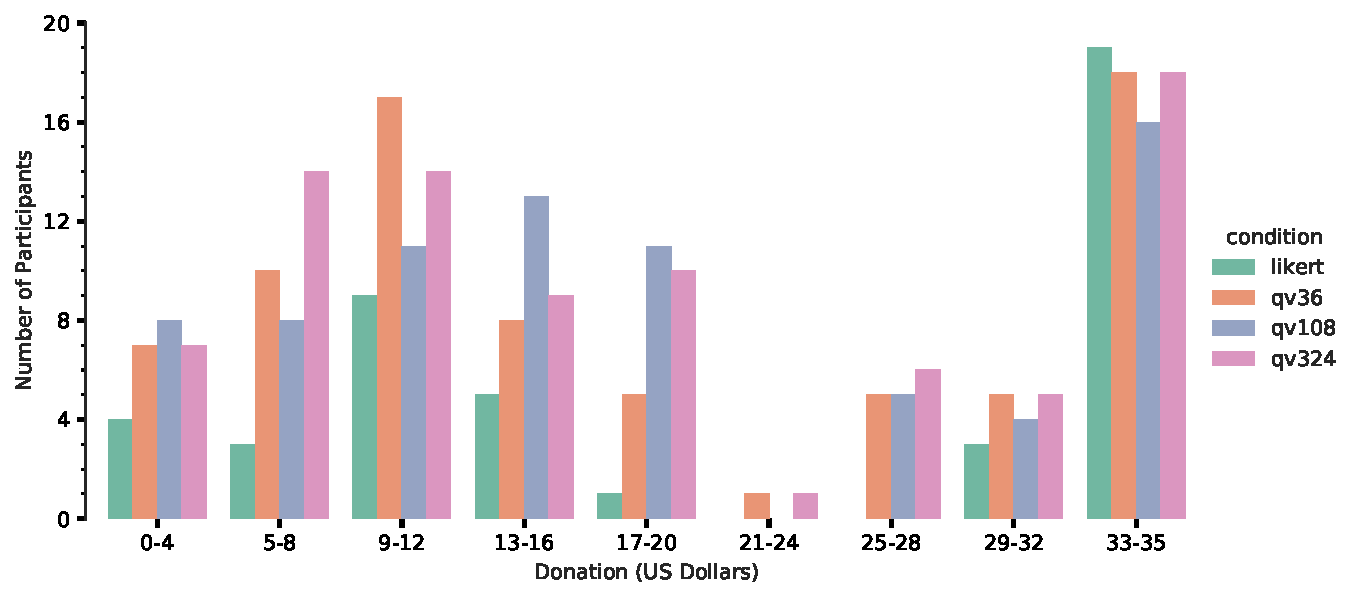
\includegraphics[width=\textwidth, keepaspectratio=true]{content/image/total_contributions_across_conditions.pdf}
    \caption{
       Distributions of the total amount donated by participants across four surveying methods.
       We saw two distributions, one centered by $\$9-12$ and the other centered by $\$33$ to $\$35$.
       We also see more Likert participants donate almost most of their donation quota compared to the QV Groups.
    }
    \Description[Distributions of Total Donation Amounts across Groups for experiment one]{ Distributions of the total amount donated by participants across four surveying methods.
    We see two distributions, one centered by $\$9-12$ and the other centered by $\$33$ to $\$35$.
    We also see more Likert participants donate almost most of their donation quota compared to the QV Groups.}
    \label{fig:total_don_exp1}
\end{figure}

\subsection{Total Donation Amount}~\label{total_donation}
Figure \ref{fig:total_don_exp1} also demonstrates two clusters for the total donation amount. The first cluster centered around $\$9-12$ with the majority in the range of $\$5-20$. This group of people, making up about $60\%$ of the entire sample, donated part of the lottery winning amount but still kept a significant portion for themselves. The other clustered around $\$33$ to $\$35$, suggesting that this group of participants
contributed almost the full amount of the lottery prize. There were approximately $25\%$ of the participants who behaved this way. The total donation amount distribution across four surveying methods were relatively consistent, except that almost twice the proportion of participants in the Likert condition donated almost the full amount compared to the other QV conditions. One possible explanation for the difference is 
the Likert group required less effort compared to that of QV, and participants felt less tempted to earn an extra reward for their time spent in the Likert condition. 

\begin{figure}[htpb]
    \centering
    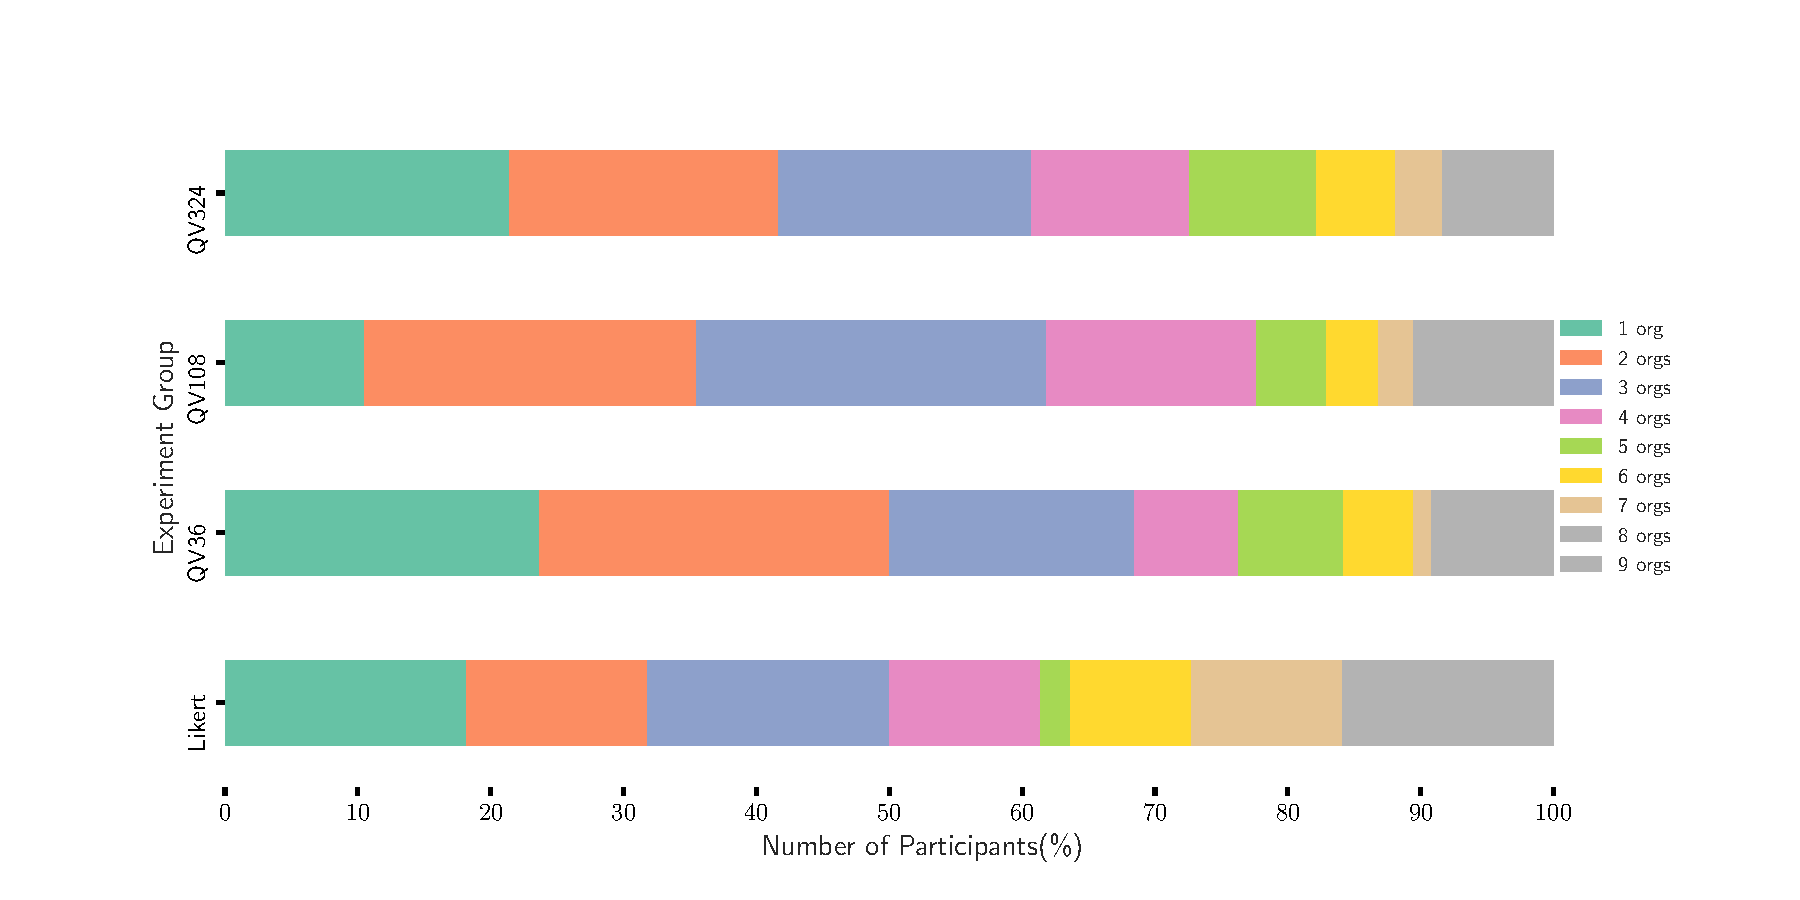
\includegraphics[width=\textwidth, keepaspectratio=true]{content/image/contribution_to_org.pdf}
    \caption{
        The distributions of how participants donated within each experiment group for experiment one. This plot removed participants that donated to zero organizations since they were excluded from our original analysis. We see that across all experiment groups, about 80\% of participants donated to more than two or more organizations. More than half of all participant donated to more than 3 organizations.
    }
    \Description[Distributions of how participants donated for experiment one]{The distributions of how participants donated within each experiment group for experiment one. This plot removed participants that donated to zero organizations since they were excluded from our original analysis. We see that across all experiment groups, about 80\% of participants donated to more than two or more organizations. More than half of all participant donated to more than 3 organizations.}
    \label{fig:par_don_exp1}
\end{figure}

\subsection{How Participants Donated}~\label{individual_donation}
To ensure that participants distributed their donation amount, we extracted the information on how each individual donated. \Cref{fig:par_don_exp1} shows the distribution of how the participants contributed to each group. On an aggregated level, only 18.57\% of participants donated to a single charity, and 59.29\% of participants donated to three or more charity.

\subsection{QV Budget Usage}
To understand how participants used their budgets, we examined the percentage of credits consumed. Participants do not need to use up all their budgets in QV. We found no decrease in the median of percentage budget usage -- all around 98\%, as available voice credits increased. QV324 did exhibit a longer tail for percentage budget usage. Participants, in general, used up their budgets as much as they can while they make trade-offs between options, under budget constraints.
\begin{figure}[htpb]
    \centering
    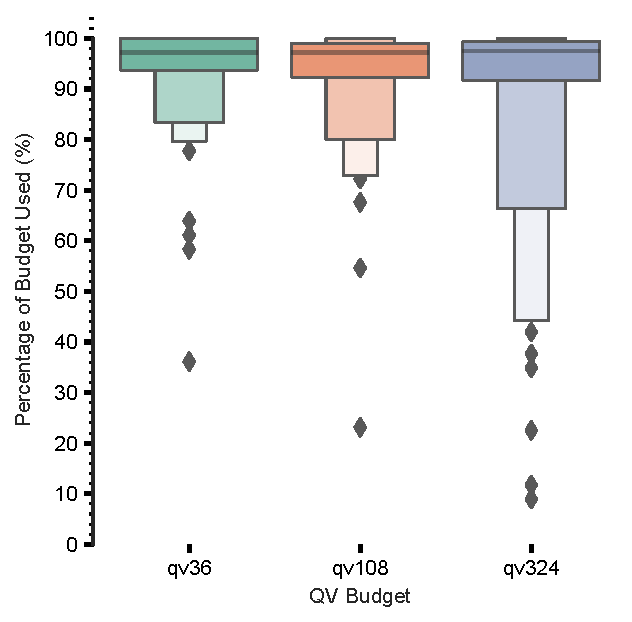
\includegraphics[width=0.5\textwidth, keepaspectratio=true]{content/image/qv_budget_used_distribution.pdf}
    \caption{
      Distribution of Percentage Budget Used in QV36, QV108 and QV324. Percentage budget used is the percentage of voice credits used out of the total voice credits budget available. The medians for all three QVs are around 98\%.
    }
    \Description[Distribution of Percentage Budget Used for experiment one]{Distribution of Percentage Budget Used for experiment one}
    \label{fig:qv_budget_exp1}
\end{figure}


\section{Experiment Two Design}
\subsection{Experiment 2 Flow Chart}
\tc{We present the experiment flow chart for experiment two in \Cref{fig:exp2_flow}. Specifically, \Cref{fig:exp2_store} provides the two interface involved for Step 6.

\begin{figure}[htpb]
    \centering
    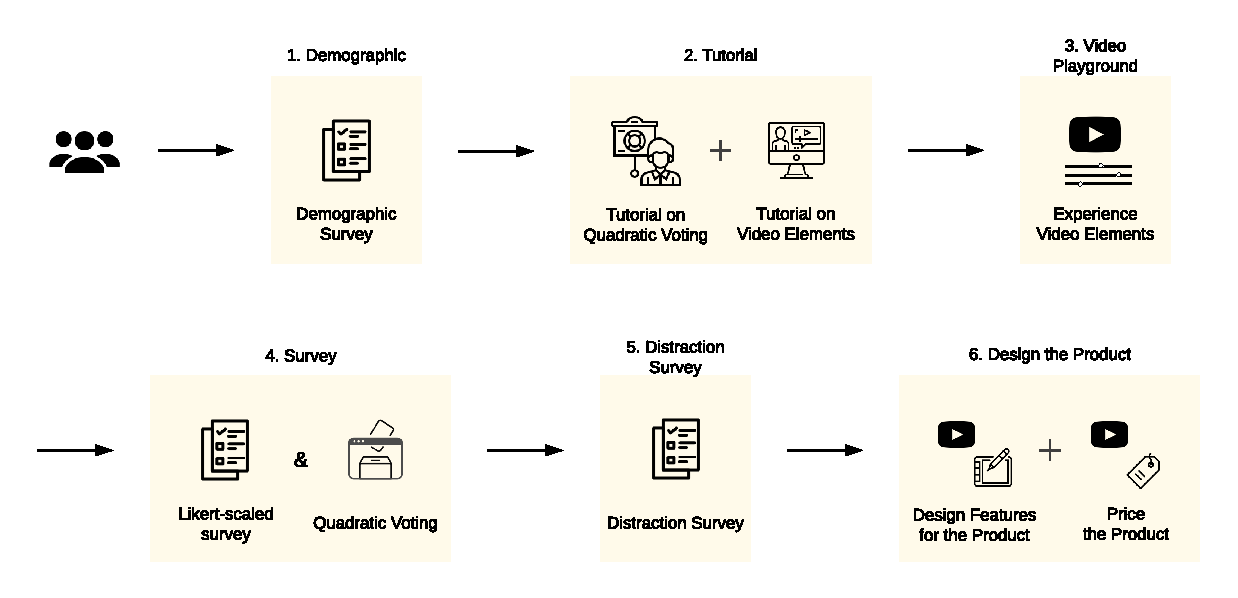
\includegraphics[width=\textwidth, keepaspectratio=true]{content/image/exp2_procedure.pdf}
    \caption{
        We used a within-subjects design for experiment two. We randomly assigned participants into two groups: one group would complete the Likert scale first and then quadratic voting; the other group experienced them in a reversed order.
    }
    \label{fig:exp2_flow}
\end{figure}

\begin{figure}[htpb]
    \centering
    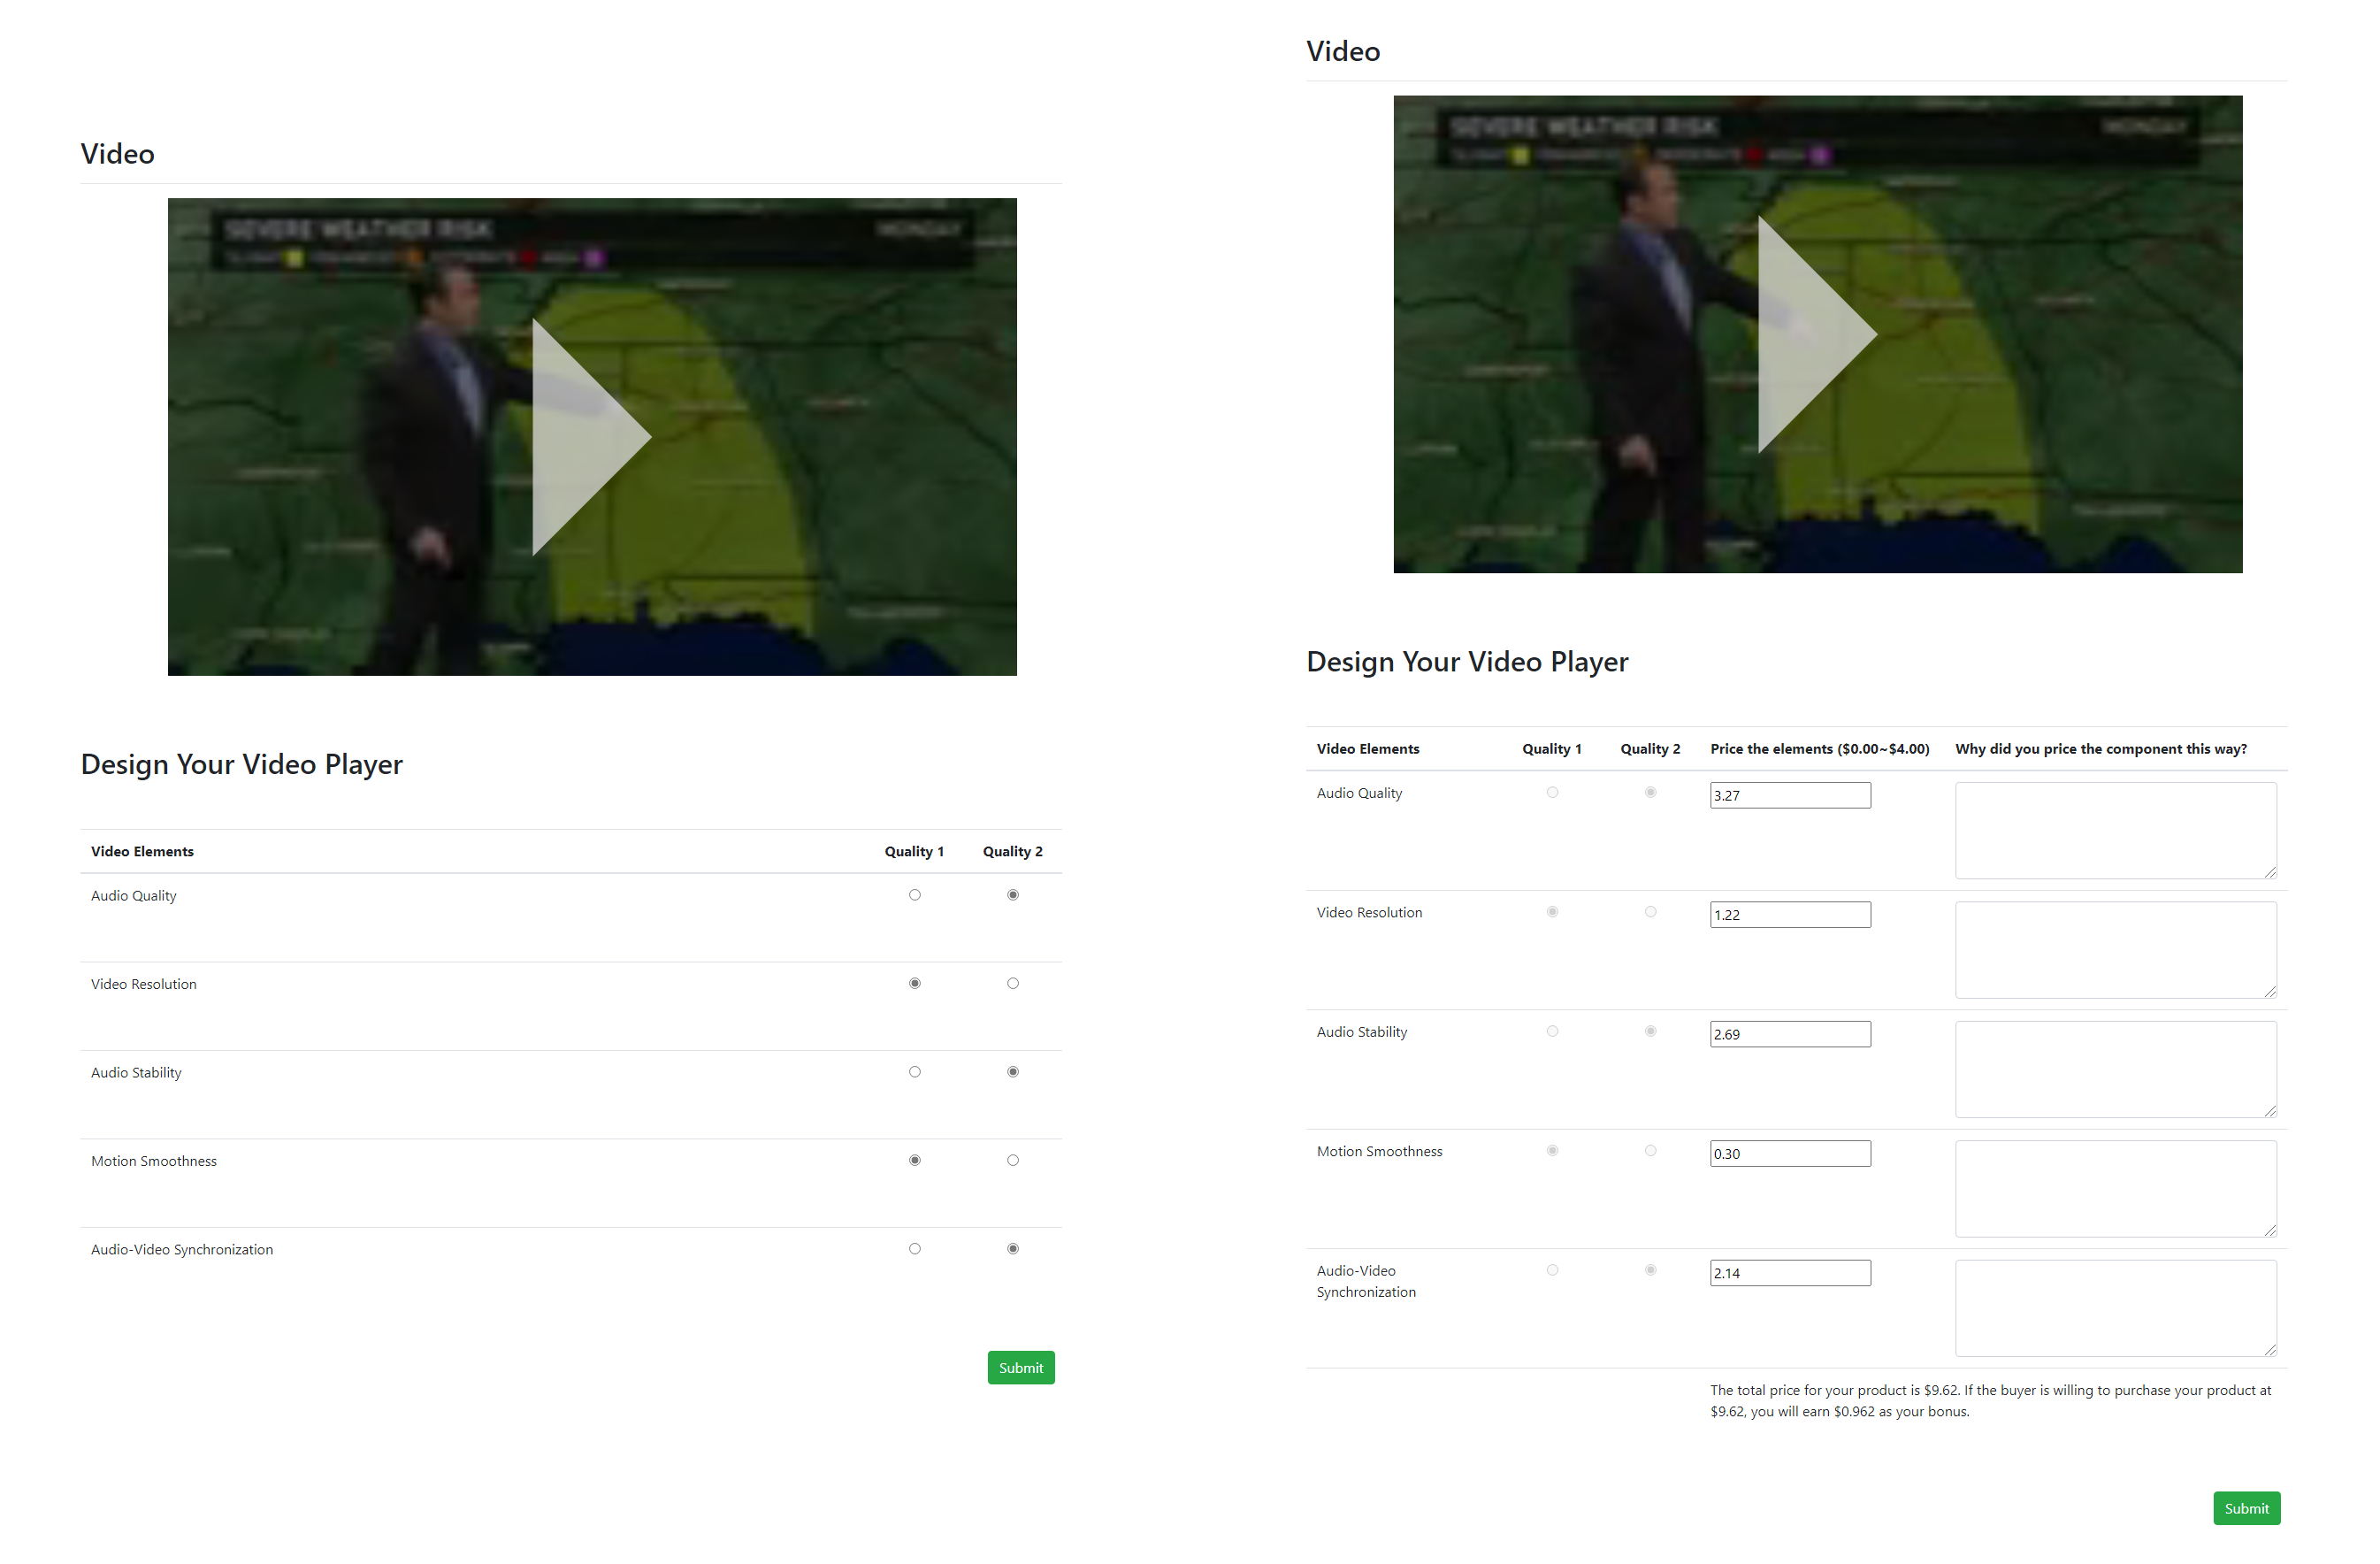
\includegraphics[width=\textwidth, keepaspectratio=true]{content/image/design_task.png}
    \caption{
        The two steps participants encountered when completing Step 6 of the survey. Participants would first need to select which one of the two qualities they would include in their video streaming product. Participants could see real-time changes to the video as they updated the qualities. Once they made their decisions, participants would price each of the elements between \$0 and \$4. Participants would receive a commission worth 10\% of the total price if the buyer accepted their product at their set prices.
    }
    \label{fig:exp2_store}
\end{figure}
}

\subsection{Definition of the Five Video Elements for Experiment Two}~\label{elem_def}
In experiment two, we designed the research scenario to answer the following question: ``Given a video with unsatisfying quality, under limited bandwidth, how should the bandwidth be allocated to enhance the five video and audio elements, including the motion smoothness \cite{huynh2008temporal}, audio stability \cite{hardman1998successful}, audio quality \cite{knoche2008low}, video resolution \cite{knoche2005can}, and audio-video synchronization \cite{steinmetz1996human}, to obtain an acceptable video streaming experience from the viewers' perspective?'' We selected the five video playback elements based on prior work, and below are their definitions: 

\begin{itemize}
    \item Motion Smoothness \cite{huynh2008temporal, oeldorf2012bad}: refers to how smooth the visuals of the video are. The number of frames transferred from the server to the viewer per second may be impacted under limited bandwidth. Having a low frame rate means that the video feels jerky and slow.
    \item Audio Stability \cite{hardman1998successful}: refers to how smoothly the audio of the video plays. With limited bandwidth, there may be lost audio packets. This creates short intervals of silence during playback, undermining the interpretability of the audio. The higher probability an audio packet may be lost, the more stuttered the audio sounds.
    \item Video Resolution \cite{oeldorf2012bad, knoche2005can}: refers to how sharp the visuals in the video look. With limited bandwidth, one may reduce the video's size by providing a lower resolution. At a lower resolution, the video imagery becomes pixelated and unclear. 
    \item Audio Quality \cite{oeldorf2012bad, noll1993wideband}: refers to how clear and crisp the audio sounds. A lower audio sampling rate needs a lower bandwidth to transmit. With a lower audio sampling rate, the audio sounds more muffled and unclear.
    \item Audio-Video Synchronization \cite{steinmetz1996human}: refers to how well video visuals are matched with the audio playback. Our experiment focused only on the type of asynchronization where the audio plays ahead of the video. Under bandwidth constraint, visuals and audio may be out of sync due to packet loss in visuals or audio.
\end{itemize}



\section{System Design Details}

\begin{figure}
     \centering
     \begin{subfigure}[ht]{0.49\textwidth}
         \centering
         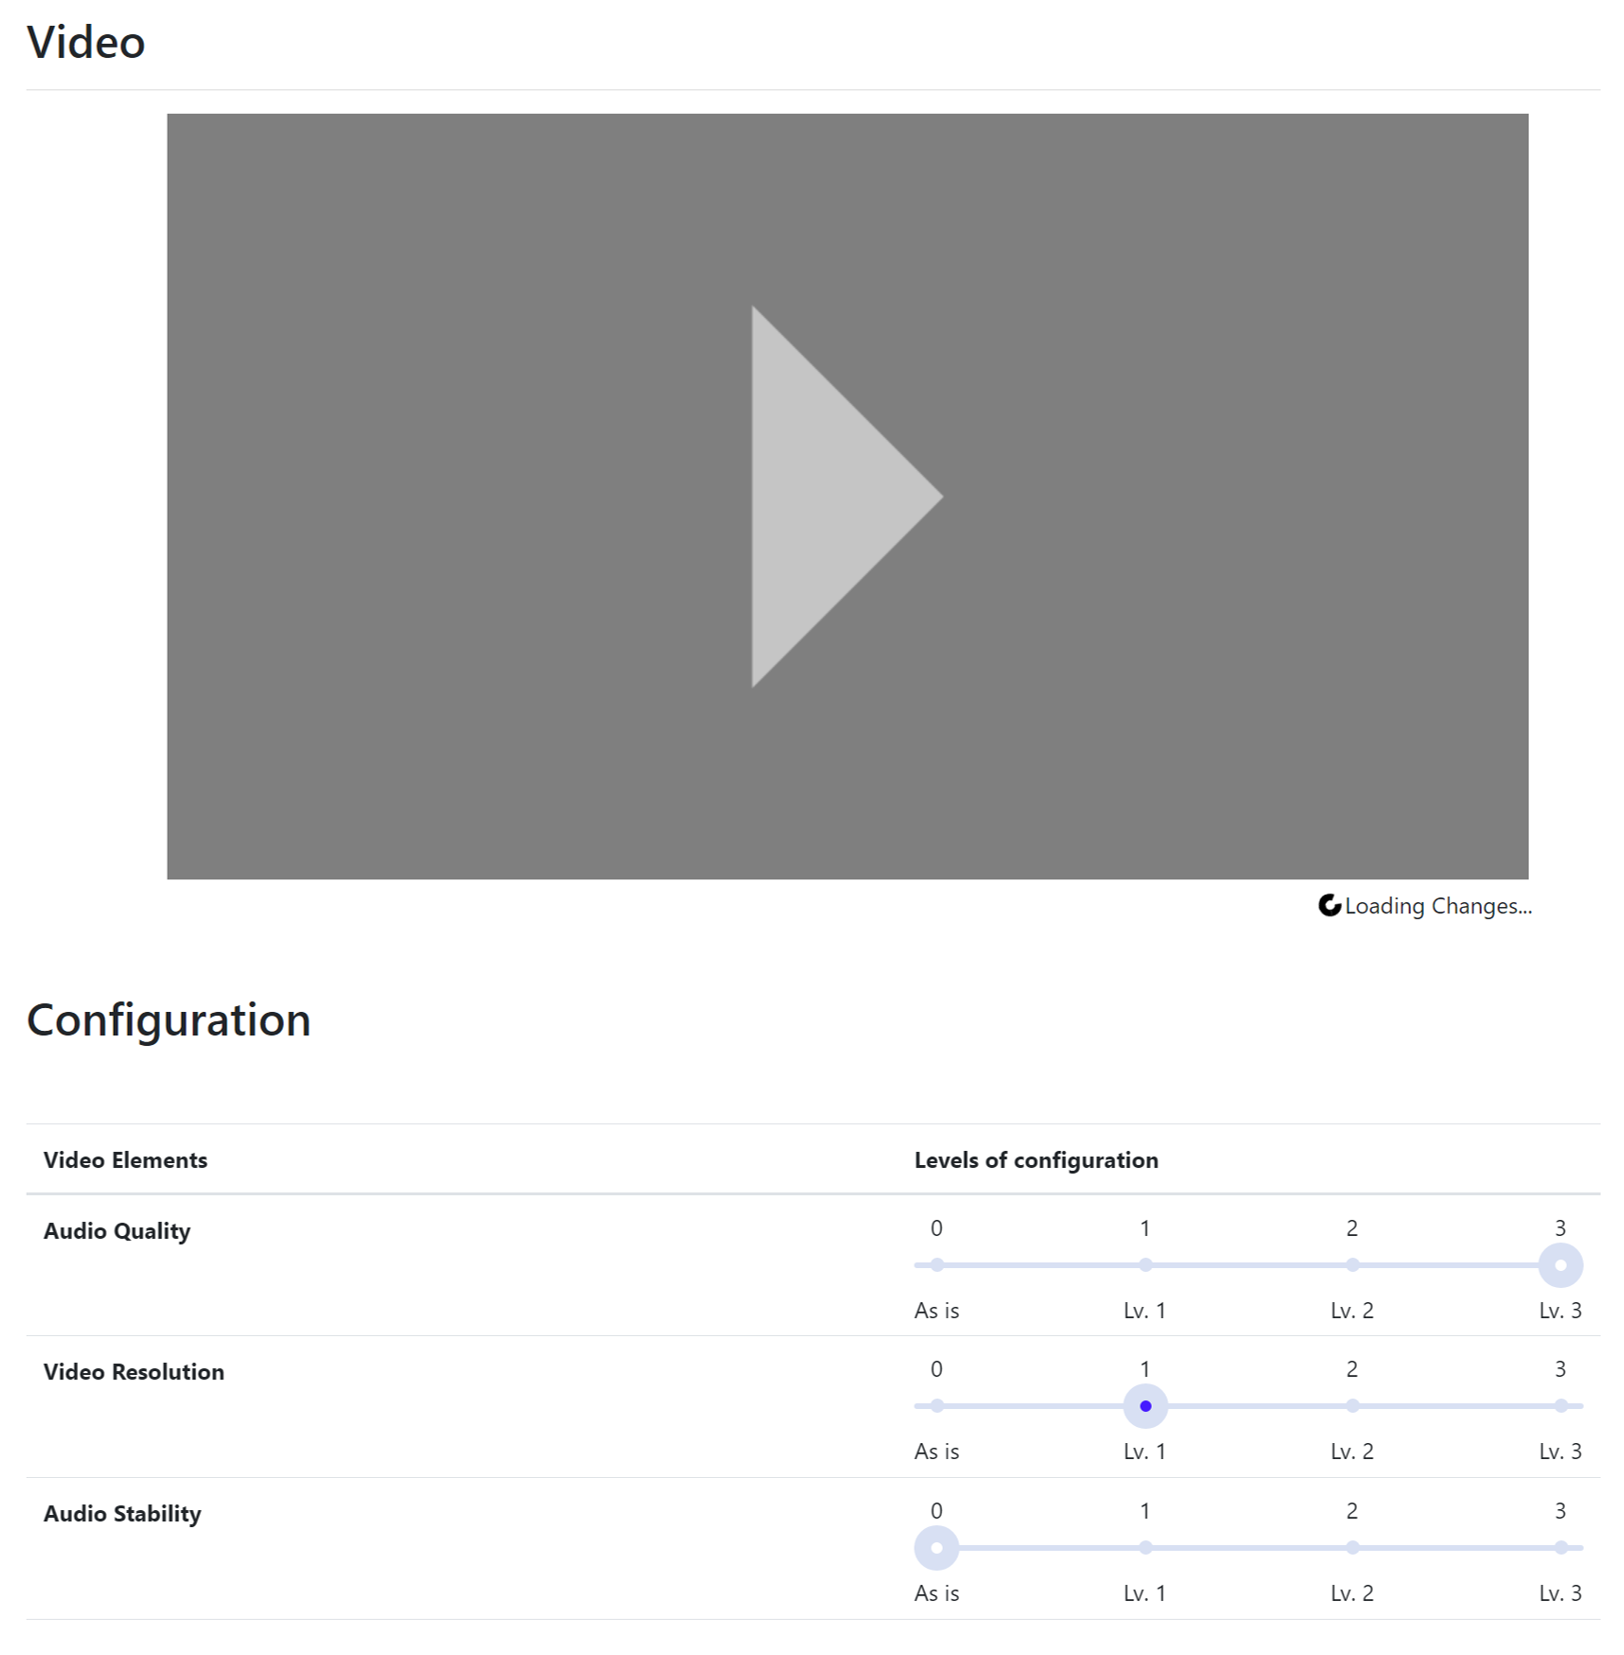
\includegraphics[width=\textwidth]{content/image/player_loading.png}
         \caption{Video interface when loading}
         \label{fig:video_loading}
     \end{subfigure}
     \hfill
     \begin{subfigure}[ht]{0.49\textwidth}
         \centering
         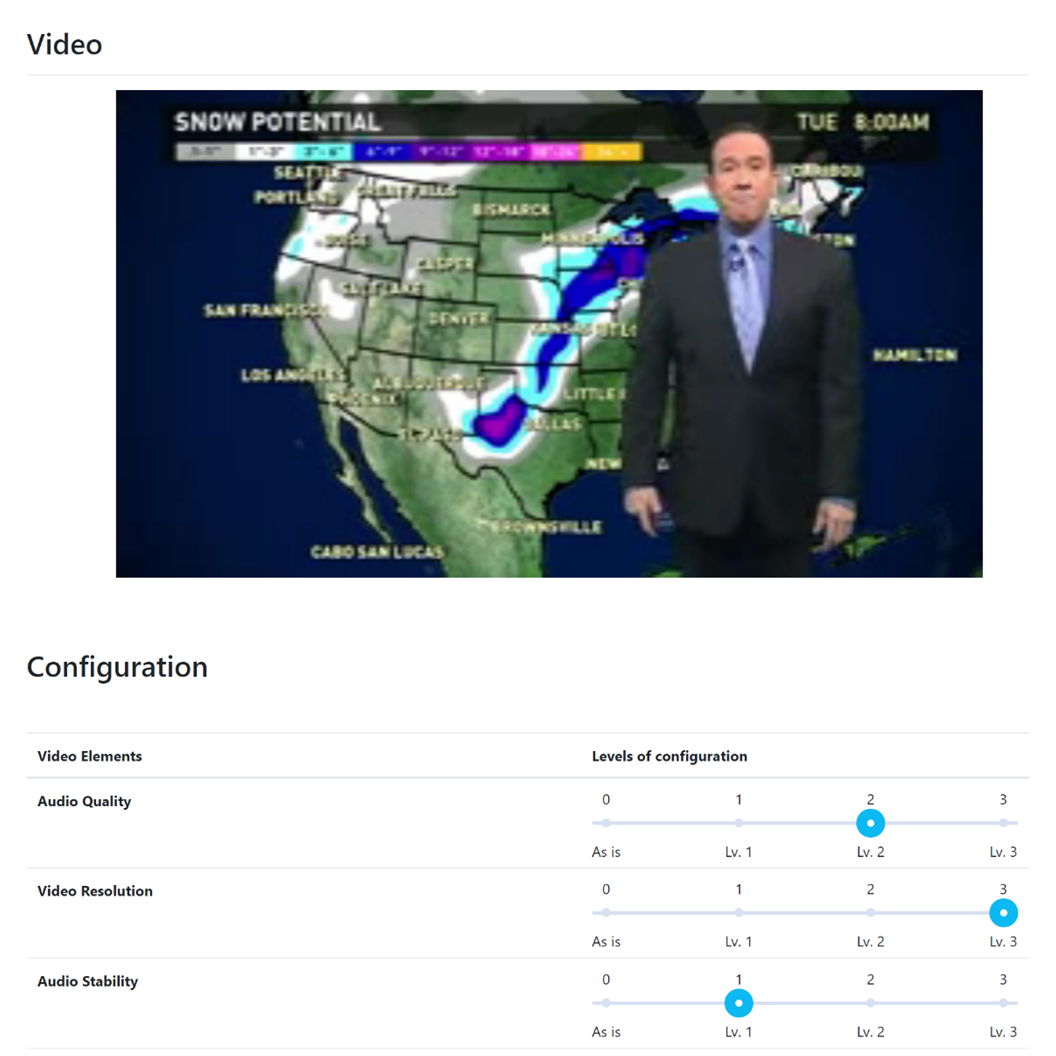
\includegraphics[width=\textwidth]{content/image/player.png}
         \caption{Video interface when playing}
         \label{fig:video_playing}
     \end{subfigure}
        \caption{To assure video playback consistency, the interface would signal loading when switching video and audio files upon participants changing the toggles. The image to the left shows how the cue was presented. The image to the right shows how the system works under normal conditions.}
        \label{fig:appendix_video_interface}
\end{figure}

\subsection{Experiment two video interface implementation detials}~\label{appx_video_interface}
For this experimental setup, we used AngularJS and bootstrap for the front-end implementation powered by Flask web framework written in Python. We used MongoDB Atlas to store data and Heroku to serve the system. Survey.js rendered all types of surveys besides the QV interface in our experiment. The experiment source code is publicly available \footnote{https://github.com/dummy\_url} and so is the standalone QV interface \footnote{https://github.com/dummy\_url}.

In this experiment, the most challenging component is to design a stable, reliable, and real-time video rendering interface for participants to experience how changes in different video element quality contribute to their overall experience. Since we provided four possible levels of adjustments for each element, there will be $4^5 = 1024$ possible combinations, which is impossible to pre-generate and serve to the participants. Therefore, we need a real-time rendering video playback system in our experiment. 

To the best of our knowledge, no video player supports real-time rendering of different video qualities ,and that there is little work that degrades video playback purposely. Thus, to achieve our experiment goal, we need to implement our own video playback system \Cref{fig:exp2_playground}. We broke the video clip into two parts: (1) a video without audio and (2) audio. In our final experiment, we pre-generated $4^2 \time 2 = 32$ files. $4^2 =16$ of which are different levels of video quality ($N=4$) and frame rates ($N=4$) while the other $4^2$ versions are  varying levels of audio quality ($N=4$) and audio stability ($N=4$). We decided not to use the server nor the browser to render the video quality or frame rates in real-time to control what the participants see even in areas of lower internet bandwidth or when there is congestion on the server. We pre-generated the audio files because of similar reasons and pre-generation made sure the locations of packet loss were consistent across participants. FFMPEG was used to generate all 16 files. Video files were first decoded and encoded at the desired resolution, bitrate and framerate. Audio files were first decoded and and encoded at the designated bit rate. We simulated audio stability by randomly losing 40 milliseconds of packets according to the probability listed in \ref{exp2-hci}.

Once these files were pre-generated, even the most distinct environment could see the same video and audio files. Understanding that network environments might delay the transmission of video and audio files, we implemented a spinning wheel in the interface to signal while the files are still loading (\Cref{fig:video_loading}). Once the client received the correct combination of files, it will play both files simultaneously according to the corresponding time anchor (\Cref{fig:video_playing}). A front-end JavaScript determined this time anchor, simulating the video-audio synchronization levels by playing the video and audio files from different start times. 

\subsection{QV interface iterations}~\label{appx_qv_interface}
The current QV interface was designed over multiple iterations. The goal of the interface is to assist participants' voting process using visual information to reduce their cognitive load. \Cref{fig:appendix_qv_interface} portraits the draft QV interface with the current design used in our experiments. Both interfaces featured a voting panel that contained a list of options to vote on. To the left of each option, participants can use the plus and minus buttons to vote for or against an option. Buttons for an item were automatically disabled if the number of voice credits remaining did not permit an additional vote for that item. 

The major difference lies in the information presented to the participants. In the new interface, we provided a bar with the proportion of voice credits contributed to that option rather than simple text under each option. Comparing the two interfaces, the new interface also allowed more description to be present under each of the options. In addition, we floated the summary panel at the bottom of the page at any time to ensure visibility, which provided information on the number of voice credits the participants have and have not used out of the total budget. Finally, we also changed the color scheme of the interface for accessibility reasons.

\begin{figure}
     \centering
     \begin{subfigure}[ht]{0.49\textwidth}
         \centering
         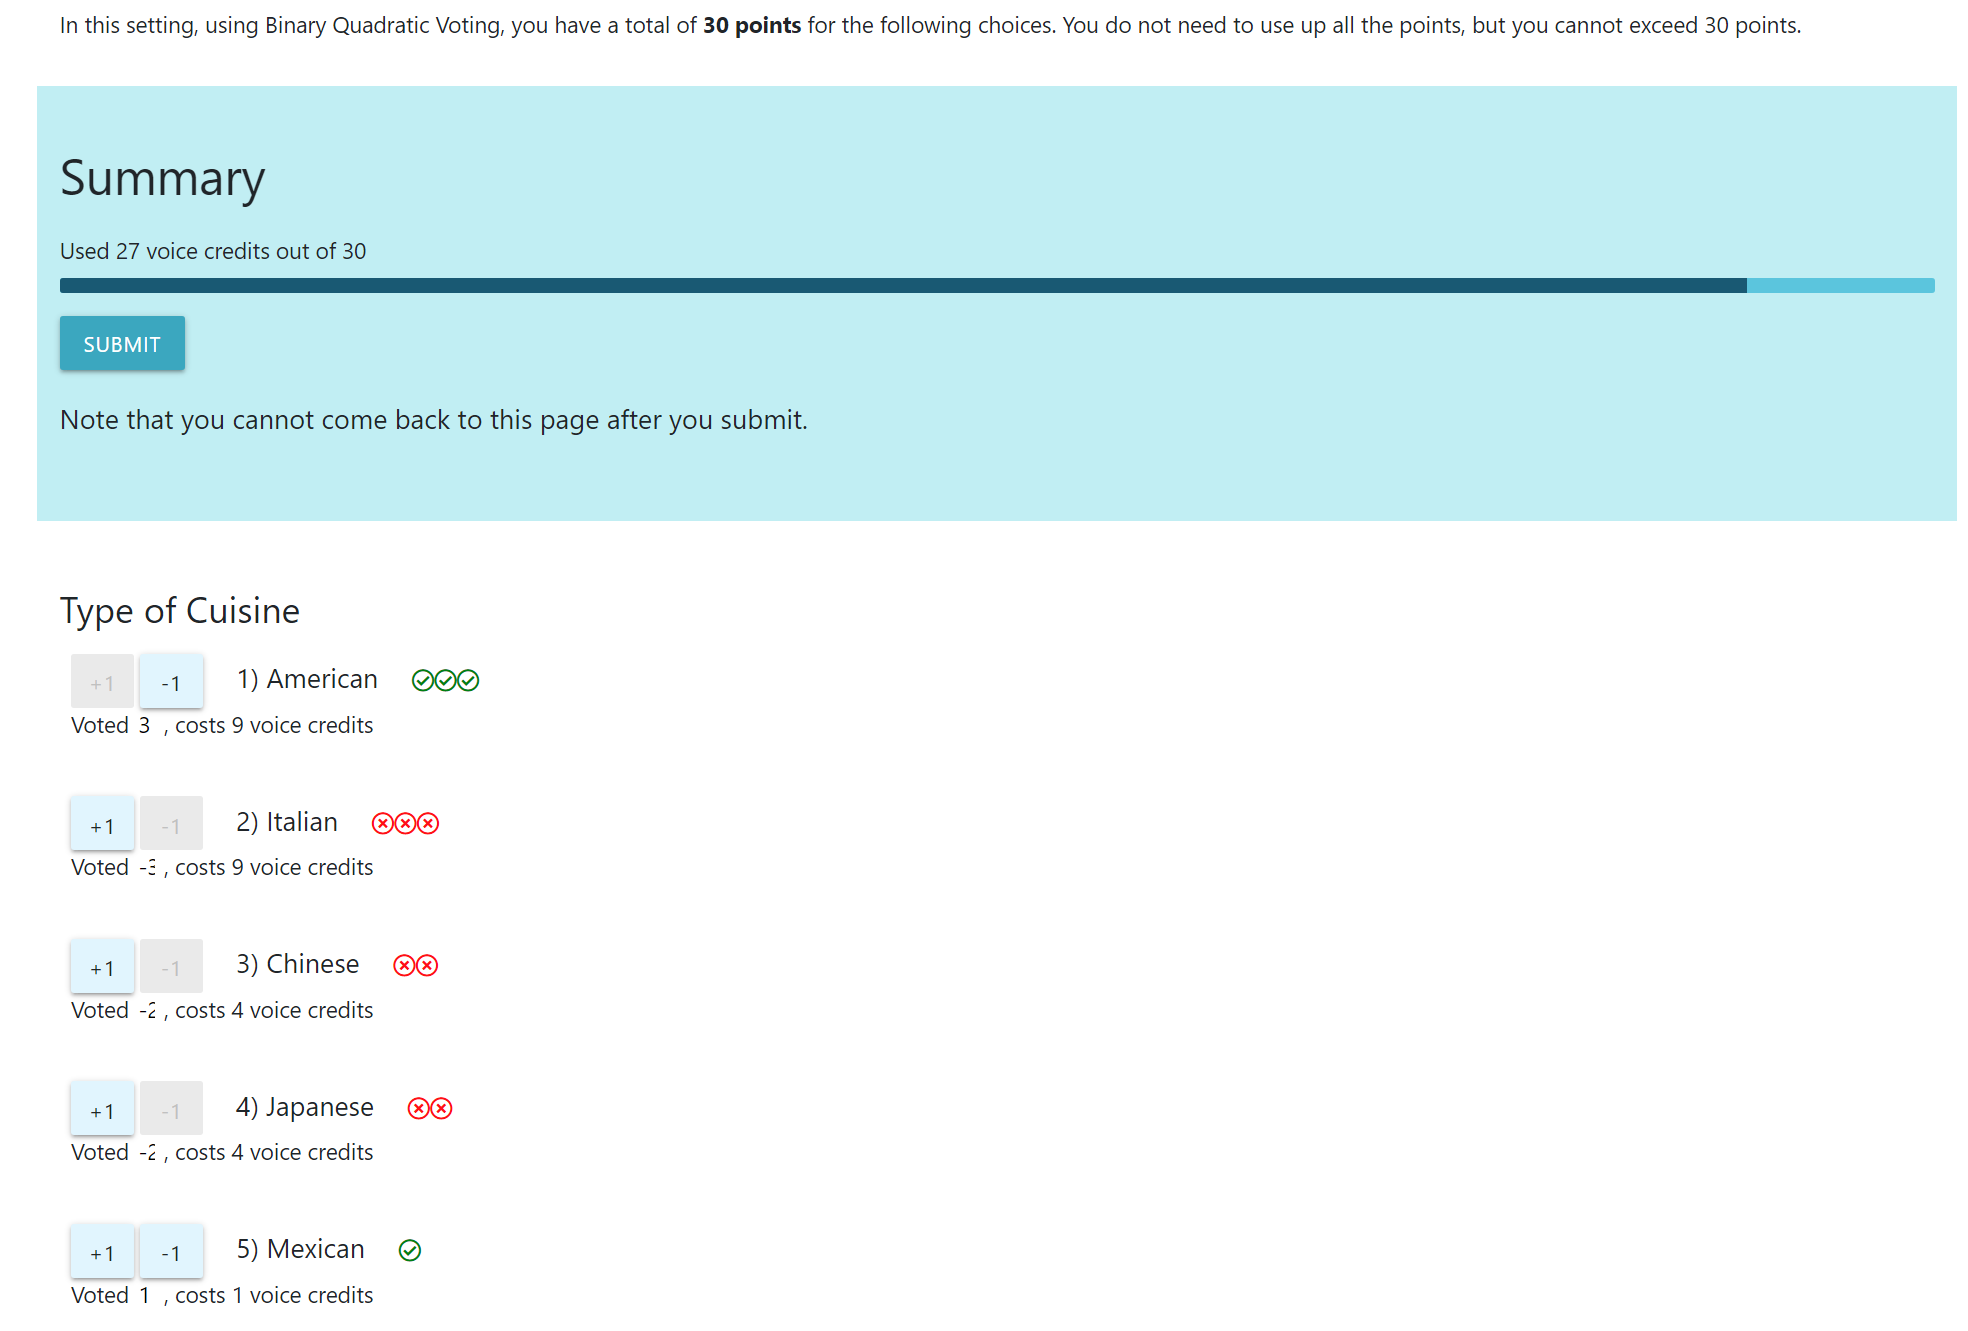
\includegraphics[width=\textwidth]{content/image/old_qv.png}
         \caption{The initial QV interface}
         \label{fig:old_qv_interface}
     \end{subfigure}
     \hfill
     \begin{subfigure}[ht]{0.49\textwidth}
         \centering
         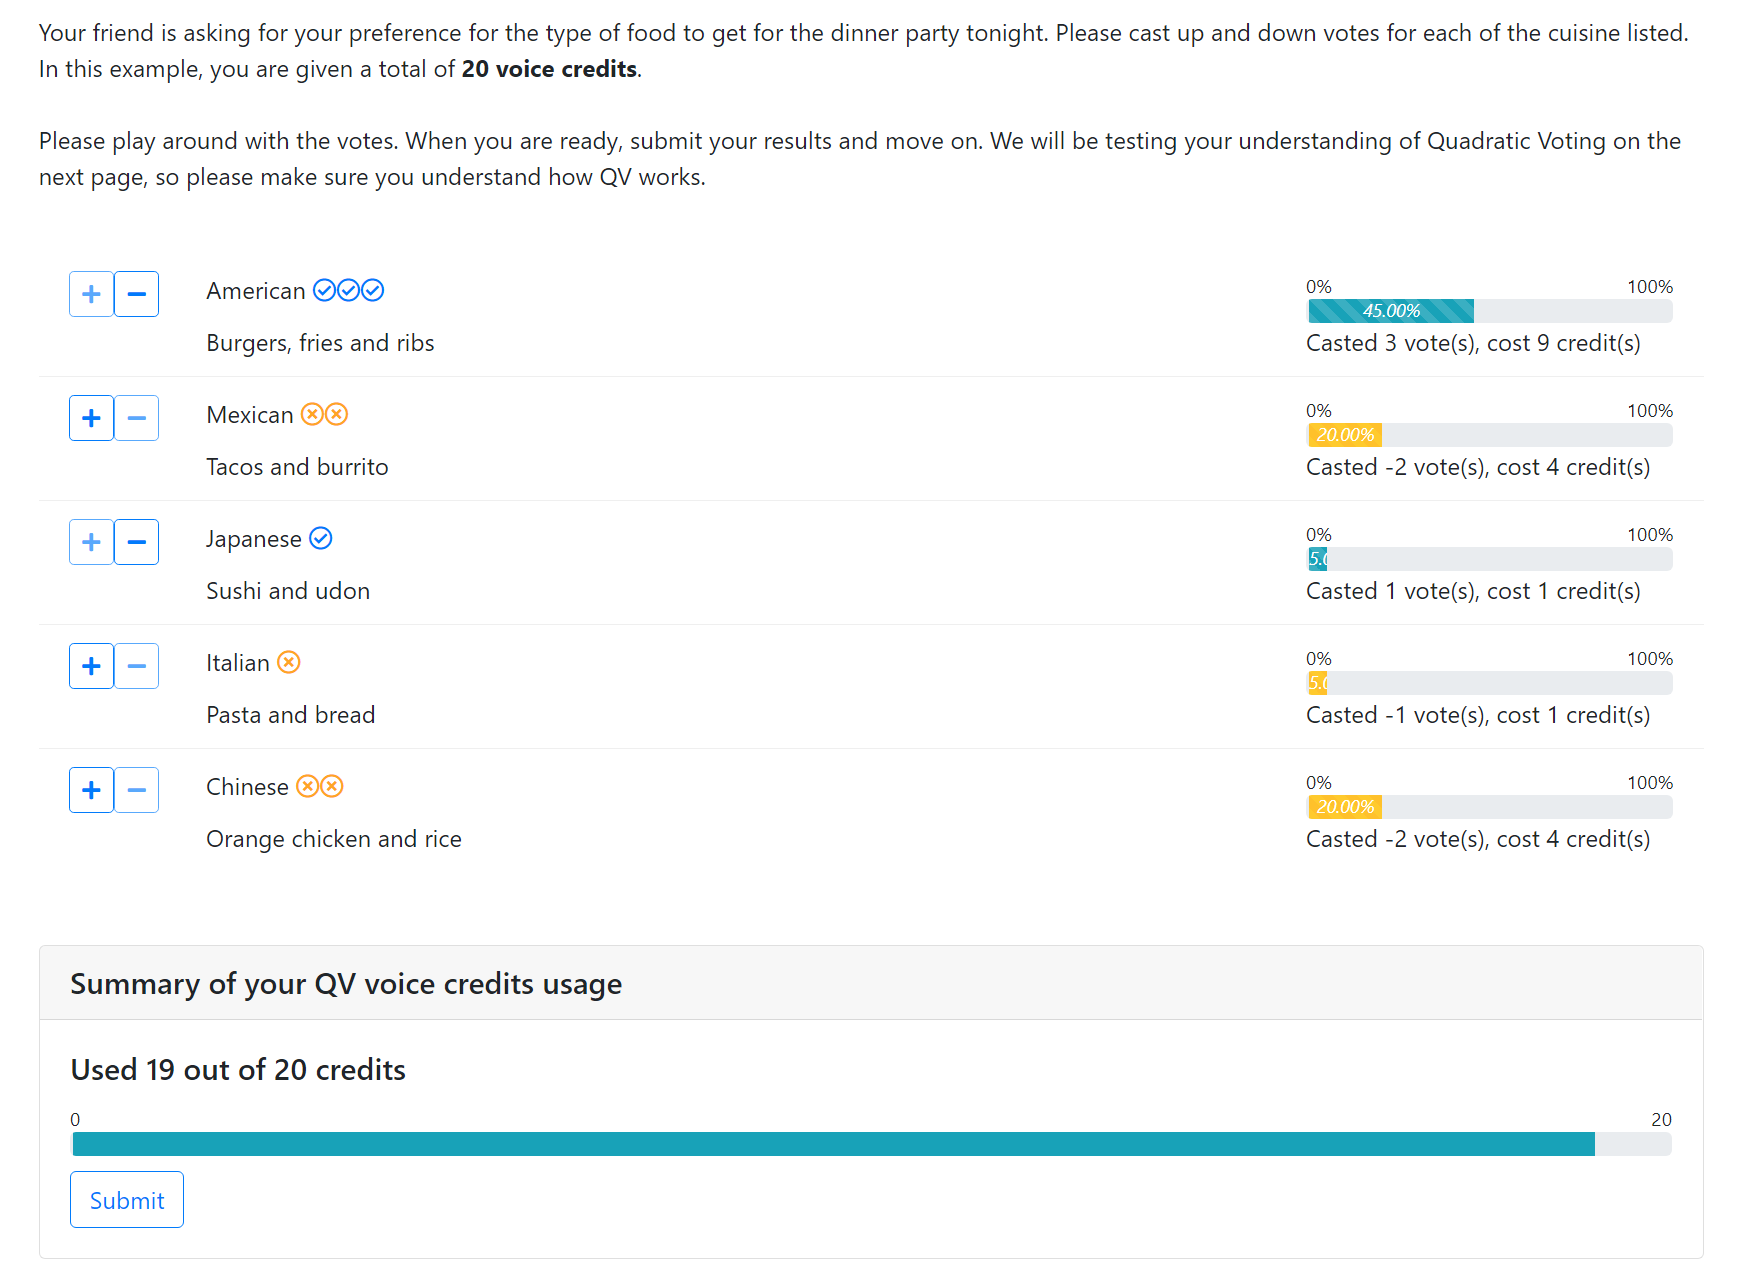
\includegraphics[width=\textwidth]{content/image/new_qv.png}
         \caption{The current QV interface}
         \label{fig:new_qv_interface}
     \end{subfigure}
        \caption{The QV interface was redesigned multiple times. The image on the left showcased the same QV playground in an early iteration of the interface design. The new design provided much more information to reduce participant's cognitive loads.}
        \label{fig:appendix_qv_interface}
\end{figure}